\chapter{Setting up interactions}
\label{sec:inter}
\newescommand{inter}
\index{interactions|mainindex}

\begin{essyntax}
  inter
\end{essyntax}

In \es, interactions are setup and investigated by the inter command. There are
mainly two types of interactions: non-bonded and bonded interactions. Non-bonded
interactions only depend on the type of the two involved particles. This also
applies to the electrostatic interaction; however, due to its long-ranged
nature, it requires special care and \es{} handles it separately with a number
of state of the art algorithms. The particle type and the charge are both
defined using the {\tt part} command.

A bonded interaction defines an interaction between a number of particles; it
however only applies to sets of particles for which it has been explicitely set.
A bonded interaction between a set of particles has to be specified explicitely
by the {\tt part bond} command, while the inter command is used to define the
interaction parameters.

Without any arguments, {\tt inter} returns a list of all defined interactions as
a Tcl-list. The format of each entry corresponds to the syntax for defining the
interaction as described below. Typically, this list looks like
\begin{tclcode}
  {0 0 lennard-jones 1.0 2.0 1.1225 0.0 0.0} {0 FENE 7.0 2.0}
\end{tclcode}

\section{Non-bonded, short-ranged interactions}
\label{sec:inter-nb}
\index{Non-bonded interactions|mainindex}
\index{interactions!non-bonded|mainindex}

\begin{essyntax}
  inter \var{type1} 
  \var{type2}
  \opt{\var{interaction}}
  \opt{\var{parameters}}
\end{essyntax}
defines an interaction of type \var{interaction} between all particles of type
\var{type1} and \var{type2}. The possible interaction types and their parameters
are listed below. If the interaction is omitted, the command returns the
currently defined interaction between the two types using the syntax to define
the interaction, \eg
\begin{tclcode}
  0 0 lennard-jones 1.0 2.0 1.1225 0.0 0.0
\end{tclcode}

For many non-bonded interactions, it is possible to artificially cap the forces,
which often allows to equilibrate the system much faster. See the
subsection~\ref{sec:forcecap} for details.

\subsection{Lennard-Jones interaction}

\index{Lennard-Jones interaction|mainindex}
\index{interactions!Lennard-Jones|mainindex}
\begin{essyntax}
  \require{1}{\variant{1}
    inter \var{type1} 
    \var{type2}
    lennard-jones 
    \var{$\epsilon$} \var{$\sigma$} 
    \var{$r_\text{cut}$} \var{$c_\text{shift}$} \var{$r_\text{off}$}
  }

  \require{2}{\variant{2}
    inter \var{type1} 
    \var{type2}
    lj-gen
    \var{$\epsilon$} \var{$\sigma$} 
    \var{$r_\text{cut}$} \var{$c_\text{shift}$} \var{$r_\text{off}$} \var{$e_1$} \var{$e_2$} 
  }
  \begin{features}
    \required[1]{LENNARD_JONES}
    \required[2]{LENNARD_JONES_GENERIC}
  \end{features}
\end{essyntax}

These two commands define a Lennard-Jones interaction between particles of the
types \var{type1} and \var{type2}.  The potential is defined by
\begin{equation}
  \label{eq:lj}
  V_\mathrm{LJ}(r) = \Biggl\{
    \begin{array}{ll}
      4\epsilon((\frac{\sigma}{r-r_\text{\var{off}}})^{e_1}
      -(\frac{\sigma}{r-r_\text{\var{off}}})^{e_2}+c_\text{\var{shift}}) 
      & \mathrm{, if~} r < r_\text{\var{cut}}+r_\text{\var{off}}\\
      \mathit{0} 
      & \mathrm{, otherwise}\\
    \end{array}.
\end{equation}
The first form of the command specifies the traditional Lennard--Jones potential
with exponents $e_1=12$ and $e_2=6$, the second form allows to choose arbitrary
exponents. Both forms allow capping the force using {\tt inter ljforcecap},
see section~\ref{sec:forcecap}.

The traditional Lennard--Jones potential is the ``work--horse'' potential for
particle--particle interactions in coarse--grained simulations. It is a simple
model for the van--der--Waals interaction, and is attractive at large distance,
but strongly repulsive at short distances. $r_\text{\var{off}} + \sigma$
corresponds to the sum of the radii of the interaction particles; at this
radius, the potential equals to $\epsilon(1+c_\text{\var{shift}})$. The
attractive part starts beyond $r=r_\text{\var{off}} + \sqrt[6]\sigma$.
\var{$r_\text{cut}$} determines from which radius on the interaction is not
calculated. Typically, one will choose the shift such that the energy is
continuous at the cutoff radius.

A special case of the Lennard--Jones potential is the Weeks--Chandler--Andersen
(WCA) potential, which one obtains by putting the cutoff into the minimum, \ie
choosing $r_\text{\var{cut}}=\sqrt[6]{2}$ and $c_\text{\var{shift}}=1/4$. The WCA
potential is purely repulsive, and is often used to mimick hard sphere repulsion.

\subsection{Lennard-Jones cosine interaction}
\index{Lennard-Jones cosine interaction|mainindex}
\index{interactions!Lennard-Jones cosine|mainindex}
\begin{essyntax}
  \variant{1}
  inter \var{type1} \var{type2} lj-cos
  \var{$\epsilon$} \var{$\sigma$}
  \var{$r_\text{cut}$} \var{$r_\text{off}$}
  \variant{2}
  inter \var{type1} \var{type2} lj-cos2
  \var{$\epsilon$} \var{$\sigma$} 
  \var{$r_\text{off}$} \var{$\omega$}
  \begin{features}
    \required[1]{LJCOS}
    \required[2]{LJCOS2}
  \end{features}
\end{essyntax}
specifies a Lennard-Jones interaction with cosine tail~\cite{soddeman01a} between
particles of the types \var{type1} and \var{type2}. The first variant behaves as
follows: Until the minimum of the Lennard-Jones potential at \var{$r_\text{min}
  = r_\text{off} + 2^{\frac{1}{6}}\sigma$}, it behaves identical to the
unshifted Lennard-Jones potential (\var{$c_\text{shift}=0$}).  Between
\var{$r_\text{min}$} and \var{$r_\text{cut}$}, a cosine is used to smoothly
connect the potential to 0, \ie
\begin{equation}
  V(r)=\frac{1}{2}\epsilon\left(cos\left[\alpha(r-r_\text{\var{off}})^2 + \beta\right]-1\right),
\end{equation}
where
\var{$\alpha = \pi\left[(r_\text{cut}-r_\text{off})^2-(r_\text{min}-r_\text{off})^2\right]^{-1}$}
and
\var{$\beta = \pi - \left(r_\text{min}-r_\text{off}\right)^2\alpha$}.

In the second variant, the cutoff radius is $r_\text{cut}=r_\text{\var{min}} +
\omega$, and the potential between $r_\text{min}$ and $r_\text{cut}$ is given by
\begin{equation}
  V(r)=\epsilon\cos^2\left[\frac{\pi}{2\omega}(r - r_\text{min})\right].
\end{equation}

Only the second variant allows capping the force using {\tt inter ljforcecap},
see section~\ref{sec:forcecap}.

\subsection{Smooth step interaction}
\index{smooth-step interaction|mainindex}
\index{interactions!smooth-step|mainindex}
\begin{essyntax}
  inter \var{type1} \var{type2}
  smooth-step \var{$\sigma_1$} \var{$n$} \var{$\epsilon$} \var{$k_0$}
  \var{$\sigma_2$} \var{$r_\text{cut}$}
  \begin{features}
    \required{SMOOTH_STEP}
  \end{features}
\end{essyntax}
This defines a smooth step interaction between particles of the
types \var{type1} and \var{type2}, for which the potential is
\begin{equation}
  V(r)= \left(\sigma_1/d\right)^n + \epsilon/(1 + \exp\left[2k_0 (r - \sigma_2)\right])
\end{equation}
for $r<r_\text{\var{cut}}$, and $V(r)=0$ elsewhere. With $n$ around 10, the
first term creates a short range repulsion similar to the Lennard-Jones
potential, while the second term provides a much softer repulsion. This
potential therefore introduces two length scales, the range of the first term,
$\sigma_1$, and the range of the second one, $\sigma_2$, where in general
$\sigma_1<\sigma_2$.

\subsection{BMHTF potential}
\index{BMHTF interaction|mainindex}
\index{interactions!BMHTF|mainindex}
\begin{essyntax}
  inter \var{type1} \var{type2}
  bmhtf-nacl \var{A} \var{B} \var{C} \var{D} \var{$\sigma$} \var{$r_\text{cut}$}
  \begin{features}
    \required{BMHTF_NACL}
  \end{features}
\end{essyntax}
This defines an interaction with the {\em short-ranged part} of the
Born-Meyer-Huggins-Tosi-Fumi potential between particles of the types
\var{type1} and \var{type2}, which is often used to simulate NaCl crystals. The
potential is as follows:
\begin{equation}
  V(r)= A\exp\left[B(\sigma - r)\right] -
  C r^{-6} - D r^{-8} + \epsilon_\text{shift},
\end{equation}
where $\epsilon_\text{shift}$ is chosen such that $V(r_\text{cut})=0$. For
\var{$r\ge r_\text{cut}$}, the $V(r)=0$.

For NaCl, the parameters should be chosen as follows:\\[.5em]
{\centering
  \begin{tabular}{r|l|l|l|l|l}
    types & $A [kJ/mol] $ & $B [\AA^{-1}]$ &
    $C [\AA^6 kJ/mol]$ & $D [\AA^8 kJ/mol]$ & $\sigma [\AA]$ \\
    \hline
    Na-Na & 25.4435 & 3.1546 &  101.1719 &    48.1771 & 2.34 \\
    Na-Cl & 20.3548 & 3.1546 &  674.4793 &   837.0770 & 2.755 \\
    Cl-Cl & 15.2661 & 3.1546 & 6985.6786 & 14031.5785 & 3.170 \\
  \end{tabular}
}\\[.5em]
The cutoff can be chosen relatively freely because the potential decays
fast; a value around 10 seems reasonable.

In addition to this short ranged interaction, one needs to add a Coulombic,
long--ranged part. If one uses elementary charges, \ie a charge of $q=+1$ for
the Na--particles, and $q=-1$ for the Cl--particles, the corresponding prefactor
of the Coulomb interaction is $\approx 1389.3549 \AA\,kJ/mol$.

\subsection{Morse interaction}
\index{Morse interaction|mainindex}
\index{interactions!Morse|mainindex}

\begin{essyntax}
  inter \var{type1} \var{type2} morse
  \var{$\epsilon$} \var{$\alpha$} \var{$r_\text{min}$} \var{$r_\text{cut}$}
  \begin{features}
    \required{MORSE}
  \end{features}
\end{essyntax}
This defines an interaction using the Morse potential between particles of the
types \var{type1} and \var{type2}. It serves similar purposes as the
Lennard-Jones potential, but has a deeper minimum, around which it is harmonic.
This models the potential energy in a diatomic molecule.  This potential allows
capping the force using {\tt inter morseforcecap}, see
section~\ref{sec:forcecap}.

For \var{$r < r_\text{cut}$}, this potential is given by
\begin{equation}
  V(r)=\epsilon\left(\exp\left[-2 \alpha \left(r - r_\text{min}\right)\right]
    - 2\exp\left[-\alpha\left(r - r_\text{min}\right)\right]\right) -
  \epsilon_\text{shift},
\end{equation}
where \var{$\epsilon_\text{shift}$} is again chosen such that
$V(r_\text{\var{cut}})=0$. For \var{$r\ge r_\text{cut}$}, the $V(r)=0$.

\subsection{Buckingham interaction}
\index{Buckingham interaction|mainindex}
\index{interactions!Buckingham|mainindex}

\begin{essyntax}
  inter \var{type1} \var{type2} buckingham
  \var{A} \var{B} \var{C} \var{D}
  \var{$r_\text{cut}$} \var{$r_\text{discont}$} \var{$\epsilon_\text{shift}$}
  \begin{features}
    \required{BUCKINGHAM}
  \end{features}
\end{essyntax}
This defines a Buckingham interaction between particles of the types
\var{type1} and \var{type2}, for which the potential is given by
\begin{equation}
  V(r)= A\exp(-B r) - Cr^{-6} - Dr^{-4} + \epsilon_\text{\var{shift}}
\end{equation}
for \var{$r_\text{discont} < r < r_\text{cut}$}. Below \var{$r_\text{discont}$},
the potential is linearly continued towards $r=0$, similarly to force capping,
see below. Above \var{$r=r_\text{cut}$}, the potential is 0. This potential
allows capping the force using {\tt inter buckforcecap}, see
section~\ref{sec:forcecap}.

\subsection{Soft-sphere interaction}
\index{soft-sphere interaction|mainindex}
\index{interactions!soft-sphere|mainindex}

\begin{essyntax}
  inter \var{type1} \var{type2}
  soft-sphere \var{a} \var{n} \var{$r_\text{cut}$} \var{$r_\text{offset}$}
  \begin{features}
    \required{SOFT_SPHERE}
  \end{features}
\end{essyntax}
This defines a soft sphere interaction between particles of the types
\var{type1} and \var{type2}, which is defined by a single power law:
\begin{equation}
  V(r)=a\left(r-r_\text{\var{offset}}\right)^{-n}
\end{equation}
for $r<r_\text{\var{cut}}$, and $V(r)=0$ above. There is no shift implemented
currently, which means that the potential is discontinuous at
$r=r_\text{\var{cut}}$. Therefore energy calculations should be used with great
caution.

\subsection{Gay-Berne interaction}
\index{Gay-Berne interaction|mainindex}
\index{interactions!Gay-Berne|mainindex}

\begin{essyntax}
  inter \var{type1} \var{type2} gay-berne
  \var{$\epsilon_0$} \var{$\sigma_0$} \var{$r_\text{cutoff}$}
  \var{k1} \var{k2} \var{$\mu$} \var{$\nu$}
  \begin{features}
    \required{ROTATION}
  \end{features}
\end{essyntax}
This defines a Gay-Berne potential for prolate and oblate particles between
particles of the types \var{type1} and \var{type2}. The Gay-Berne potential is
an anisotropic version of the classic Lennard-Jones potential, with
orientational dependence of the range $\sigma$ and the well-depth $\epsilon$.

Assume two particles with orientations given by the unit vectors
$\mathbf{\hat{u}}_i$ and $\mathbf{\hat{u}}_j$ and intermolecular vector
$\mathbf{r} = r\mathbf{\hat{r}}$. If $r<r_\text{\var{cut}}$, then the
interaction between these two particles is given by
\begin{equation}
  V(\mathbf{r}_{ij}, \mathbf{\hat{u}}_i, \mathbf{\hat{u}}_j) = 4
  \epsilon(\mathbf{\hat{r}}_{ij}, \mathbf{\hat{u}}_i,
  \mathbf{\hat{u}}_j) \left( \tilde{r}_{ij}^{-12}-\tilde{r}_{ij}^{-6}
  \right),
\end{equation}
otherwise $V(r)=0$. The reduced radius is
\begin{equation}
  \tilde{r}=\frac{r - \sigma(\mathbf{\hat{r}},
    \mathbf{\hat{u}}_i, \mathbf{\hat{u}}_j)+\sigma_0}{\sigma_0},
\end{equation}
\begin{equation}
  \sigma( \mathbf{\hat{r}}, \mathbf{\hat{u}}_i,
  \mathbf{\hat{u}}_j) = \sigma_{0} \left\{ 1 - \frac{1}{2} \chi \left[
      \frac{ \left( \mathbf{\hat{r}} \cdot \mathbf{\hat{u}}_i +
          \mathbf{\hat{r}} \cdot \mathbf{\hat{u}}_j \right)^{2} }
      {1 + \chi \mathbf{\hat{u}}_i \cdot \mathbf{\hat{u}}_j } +
      \frac{ \left( \mathbf{\hat{r}} \cdot \mathbf{\hat{u}}_i -
          \mathbf{\hat{r}} \cdot \mathbf{\hat{u}}_j \right)^{2} }
      {1 - \chi \mathbf{\hat{u}}_i \cdot \mathbf{\hat{u}}_j}
    \right] \right\}^{-\frac{1}{2}}
\end{equation}
and
\begin{multline}
  \epsilon(\mathbf{\hat{r}}, \mathbf{\hat{u}}_i,
  \mathbf{\hat{u}}_j) = \\
  \epsilon_0 \left( 1- \chi^{2}(\mathbf{\hat{u}}_i
    \cdot \mathbf{\hat{u}}_j) \right)^{-\frac {\nu}{2}} \left[1-\frac
    {\chi'}{2} \left( \frac { (\mathbf{\hat{r}} \cdot
        \mathbf{\hat{u}}_i+ \mathbf{\hat{r}} \cdot
        \mathbf{\hat{u}}_j)^{2}} {1+\chi' \, \mathbf{\hat{u}}_i \cdot
        \mathbf{\hat{u}}_j }+ \frac {(\mathbf{\hat{r}} \cdot
        \mathbf{\hat{u}}_i-\mathbf{\hat{r}} \cdot
        \mathbf{\hat{u}}_j)^{2}} {1-\chi' \, \mathbf{\hat{u}}_i \cdot
        \mathbf{\hat{u}}_j } \right) \right]^{\mu}.
\end{multline}
The parameters $\chi = \left(k_1^{2} - 1\right)/\left(k_1^{2} + 1\right)$ and
$\chi' = \left(k_2^{1/\mu} - 1\right)/\left(k_2^{1/\mu} + 1\right)$ are
responsible for the degree of anisotropy of the molecular properties.
\var{$k_1$} is the molecular elongation, and \var{$k_2$} is the ratio of the
potential well depths for the side-by-side and end-to-end configurations.  The
exponents $ \mu $ and $ \nu $ are adjustable parameters of the potential.
Several Gay-Berne parametrizations exist, the original one being $k_1 = 3$,
$k_2 = 5$, $\mu = 2$ and $\nu = 1$.

\subsection{Tabulated interaction}
\index{tabulated interaction|mainindex}
\index{interactions!tabulated|mainindex}
\label{sec:tabnonbonded}

\begin{essyntax}
  inter \var{type1} \var{type2} tabulated \var{filename}%
  \begin{features}
    \required{TABULATED}
  \end{features}
\end{essyntax}

This defines an interaction between particles of the types \var{type1} and
\var{type2} according to an arbitrary tabulated pair potential. \var{filename}
specifies a file which contains the tabulated forces and energies as a function
of the separation distance. The tabulated potential allows capping the force
using {\tt inter tabforcecap}, see section~\ref{sec:forcecap}.

At present the required file format is simply an ordered list separated by
whitespace. The data reader first looks for a {\tt \#} character and begins
reading from that point in the file. Anything before the {\tt \#} will be
ignored.

The first three parameters after the {\tt \#} specify the number of data points
$N_\text{points}$ and the minimal and maximal tabulated separation distances
$r_\text{min}$ and $r_\text{max}$. The number of data points obviously should
be an integer, the two other can be arbitrary positive doubles. Take care when
choosing the number of points, since a copy of each lookup table is kept on each
node and must be referenced very frequently. The maximal tabulated separation
distance also acts as the effective cutoff value for the potential.

The remaining data in the file should consist of n data triples $r$, $F(r)$ and
$V(r)$. $r$ gives the particle separation, $V(r)$ specifies the interaction
potential, and $F(r)= -V'(r)/r$ the force (note the factor $1/r$!). The values
of $r$ are assumed to be equally distributed between $r_\text{min}$ and
$r_\text{max}$ with a fixed distance of
$(r_\text{max}-r_\text{min})/(N_\text{points}-1)$; the distance values $r$ in
the file are ignored and only included for human readability.

\subsection{Capping the force during warmup}
\label{sec:forcecap}

\begin{essyntax}
  \variant{1} inter ljforcecap    \var{$F_\text{max}$}
  \variant{2} inter morseforcecap \var{$F_\text{max}$}
  \variant{3} inter buckforcecap  \var{$F_\text{max}$}
  \variant{4} inter tabforcecap   \var{$F_\text{max}$}
  \begin{features}
    \required[1]{LENNARD_JONES}
    \required[2]{MORSE}
    \required[3]{BUCKINGHAM}
    \required[4]{TABULATED}
  \end{features}  
\end{essyntax}

Non-bonded interactions are often used to model the hard core repulsion between
particles. Most of the potentials in the section are therefore singular at zero
distance, and forces usually become very large for distances below the particle
size. This is not a problem during the simulation, as particles will simply
avoid overlapping. However, creating an initial dense random configuration
without overlap is often difficult.

By artificially capping the forces, it is possible to simulate a system with
overlaps. By gradually raising the cap value $F_\text{max}$, possible overlaps
become unfavorable, and the system equilibrates to a overlap free configuration.

This command will cap the force to $F_\text{\var{max}}$, \ie for particle
distances which would lead to larger forces than $F_\text{\var{max}}$, the force
remains at $F_\text{\var{max}}$. Accordingly, the potential is replaced by
replaced by $r F_\text{\var{max}}$. Particles placed exactly on top of each other
will be subject to a force of magnitude $F_\text{\var{max}}$ along the first
coordinate axis.

The force capping is switched off by setting $F_\text{\var{max}}=0$. Note that
force capping always applies to all interactions of the corresponding type (\eg
all Lennard-Jones interactions) regardless of the particle types.

\section{Bonded interactions}
\label{sec:inter-bonded}
\index{bonded interactions|mainindex}
\index{interactions!bonded|mainindex}

\begin{essyntax}
  inter \var{bond_type_number}
  \opt{\var{interaction}}
  \opt{\var{parameters}}
\end{essyntax}

\index{bonded interaction type id} Bonded interactions are identified by their
\emph{bonded interaction type identificator} \var{bond_type_number}, which is a
non-negative integer.  The \texttt{inter} \var{bond_type_number} command is used
to specify the type and parameters of a bonded interaction, which applies to all
particles connected explicitely by this bond using the \texttt{part} command
(see section \vref{tcl:part}).  Therefore, defining a bond between two particles
always involves two steps: defining the interaction and applying it. Assuming
that two particles with ids 42 and 43 already exist, one can create \eg a
FENE-bond between them using
\begin{tclcode}
  inter 1 fene 10.0 2.0
  part 42 bond 1 43
\end{tclcode}
If a FENE-bond with the same interaction parameters is required between several
particles (\eg in a simple chain molecule), one can use the sampe type \var{id}:
\begin{tclcode}
  inter 1 fene 10.0 2.0
  part 42 bond 1 43; part 43 bond 1 44 
\end{tclcode}

Bonds can have more than just two bond partners. For the \texttt{inter} command
that does not play a role as it only specifies the parameters, only when
applying the bond using the \texttt{bond} particle, the number of involved
particles plays a role. The number of involved particles and their order, if
important, is nevertheless specified here for completeness.

\subsection{FENE bond}
\index{FENE bond|mainindex}
\index{interactions!FENE|mainindex}

\begin{essyntax}
  inter \var{bond_type_number}
  fene
  \var{$K$} \var{$R$}
\end{essyntax}
This creates a bond type with identificator \var{bond_type_number} with a FENE
(finite extension nonlinear expander) interaction. This is a rubber-band-like,
symmetric interaction betweeen two particles with prefactor $K$, and maximal
distance $R$, \ie the bond potential diverges at a particle distance $r=R$. It
is given by
\begin{equation}
  V(r) = -\frac{1}{2} K R^2\ln \left[ 1 - \left( \frac{r}{R} \right)^2 \right].
\end{equation}

\subsection{Harmonic bond}
\index{harmonic bond|mainindex}
\index{interactions!harmonic|mainindex}

\begin{essyntax}
  inter \var{bond_type_number}
  harmonic \var{K} \var{R}
\end{essyntax}
This creates a bond type with identificator \var{bond_type_number} with a
classical harmonic potential. It is a symmetric interaction between two
particles. The potential is minimal at particle distance $r=R$, and the
prefactor is $K$. It is given by
\begin{equation}
  V(r) = \frac{1}{2} K \left( r - R \right)^2
\end{equation}

\subsection{Subtracted Lennard-Jones bond}
\index{subtracted Lennard-Jones bond|mainindex}
\index{interactions!subtracted Lennard-Jones|mainindex}

\begin{essyntax}
  inter \var{bond_type_number}
  subt_lj
  \var{reserved} \var{R}
\end{essyntax}
This creates a ``bond'' type with identificator \var{bond_type_number}, which
acts between two particles and actually subtracts the Lennard-Jones interaction
between the involved particles.  The first parameter, \var{reserved} is a dummy
just kept for compatibility reasons. The second parameter, \var{R}, is used as a
check: if any bond length in the system exceeds this value, the program
terminates. When using this interaction, it is worthwhile to consider
capping the Lennard-Jones potential appropriately so that round-off errors can
be avoided.

This interaction is useful when using other bond potentials which already
include the short--ranged repulsion. This often the case for force fields or in
general tabulated potentials.

\subsection{Bond-angle interactions}
\index{bond-angle interactions|mainindex}
\index{interactions!bond-angle|mainindex}
\label{sec:angle}

\begin{essyntax}
  inter \var{bond_type_number}
  angle \var{K} \opt{\var{$\phi_0$}}
  \begin{features}
    BOND_ANGLE_HARMONIC, BOND_ANGLE_COSINE or\\
    BOND_ANGLE_COSSQUARE
  \end{features}
\end{essyntax}

This creates a bond type with identificator \var{bond_type_number} with an angle
dependent potential. This potential is defined between three particles. The
particle for which the bond is created, is the central particle, and the angle
$\phi$ between the vectors from this particle to the two others determines the
interaction.  $K$ is the bending constant, and the optional parameter
\var{$phi_0$} is the equilibirum bond angle in radiants ranging from 0 to $\pi$.
If this parameter is not given, it defaults to \var{$\phi_0 = \pi$}, which
corresponds to a stretched configuration. For example, for a bond defined by
\begin{center}
  \tt part $p_2$ bond 4 $p_1$ $p_3$
\end{center}
the following minimal energy configurations are
\begin{center}
  \setlength{\unitlength}{3000sp}
  \begin{picture}(8381,2684)(1570,-5393)
    \thinlines
    \put(2701,-4561){\circle*{450}}
    \put(3601,-4561){\circle*{450}}
    \put(4501,-4561){\circle*{450}}
    \put(7021,-4561){\circle*{450}}
    \put(7921,-4561){\circle*{450}}
    \put(7921,-3661){\circle*{450}}
    \thicklines
    \put(2701,-4561){\line( 1, 0){1800}}
    \put(7021,-4561){\line( 1, 0){900}}
    \put(7921,-4561){\line( 0, 1){900}}
    \put(5761,-2831){\line( 0,-1){2500}}

    \put(2701,-5191){\makebox(0,0)[b]{$p_1$}}
    \put(3601,-5191){\makebox(0,0)[b]{$p_2$}}
    \put(4501,-5191){\makebox(0,0)[b]{$p_3$}}
    \put(7021,-5191){\makebox(0,0)[b]{$p_1$}}
    \put(8371,-3751){\makebox(0,0)[b]{$p_3$}}
    \put(7921,-5191){\makebox(0,0)[b]{$p_2$}}
    \put(7921,-2941){\makebox(0,0)[b]{\texttt{inter 4 angle 1.0 1.57}}}
    \put(3601,-2941){\makebox(0,0)[b]{\texttt{inter 4 angle 1.0 3.14}}}
  \end{picture}%
\end{center}

For the potential acting between the three particles, different choices are
possible, which have to be activated in \texttt{myconfig.h}
\begin{itemize}
\item Harmonic bond angle potential (requires feature BOND_ANGLE_HARMONIC):\\
  A classical harmonic potential,
  \begin{equation}
    V(\alpha) = \frac{K}{2} \left(\phi - \phi_0\right)^2.
  \end{equation}
  Unlike the two following variants, this potential has a kink at
  $\phi=\phi_0+\pi$ and accordingly a discontinuity in the force, and should
  therefore be used with caution.
\item Cosine bond angle potential (requires feature BOND_ANGLE_COSINE):\\
  \begin{equation}
    V(\alpha) = K \left[1 - \cos(\phi - \phi0)\right]
  \end{equation}
  Around $\phi_0$, this potenial is close to a harmonic one (both are
  $1/2(\phi-\phi_0)^2$ in leading order), but it is periodic and smooth for all
  angles $\phi$.
\item Cosine square bond angle potential (requires feature
  BOND_ANGLE_COSSQUARE):\\
  \begin{equation}
    V(\alpha) = \frac{K}{2} \left[\cos(\phi) - \cos(\phi_0)\right]^2
  \end{equation}
  This form is used for example in the GROMOS96 force field. The potential is
  $1/8(\phi-\phi_0)^4$ around $\phi_0$, and therefore much flatter than the
  two potentials before.
\end{itemize}

\subsection{Dihedral interactions}
\index{dihedral interactions|mainindex}
\index{interactions!dihedral|mainindex}
\label{sec:dihedral}

\begin{essyntax}
  inter \var{bond_type_number}
  dihedral \var{n} \var{K} \var{$\phi$}
\end{essyntax}

This creates a bond type with identificator \var{bond_type_number} with a
dihedral potential, \ie a four-body-potential. In the followin, let the particle
for which the bond is created be particle $p_2$, and the other bond partners
$p_1$, $p_3$, $p_4$, in this order, \ie \texttt{part $p_2$ bond bond_type_number
  $p_1$ $p_3$ $p_4$}. Then the dihedral potential is given by
\begin{equation}
  V(r) = K\left[1 + \phi\,\cos(n\phi)\right],
\end{equation}
where \var{n} is the multiplicity of the potential (number of minimas) and can
take integer values from 1 to 6, \var{phi} is a phase parameter which takes the
values $\pm1$ and \var{K} is the bending constant of the potential. $\phi$ is
the dihedral angle between the particles defined by the particle quadrupel
$p_1$, $p_2$, $p_3$ and $p_4$, \ie the angle between the planes defined by the
particle triples $p_1$, $p_2$ and $p_3$ and $p_2$, $p_3$ and $p_4$, \ie
\begin{center}
  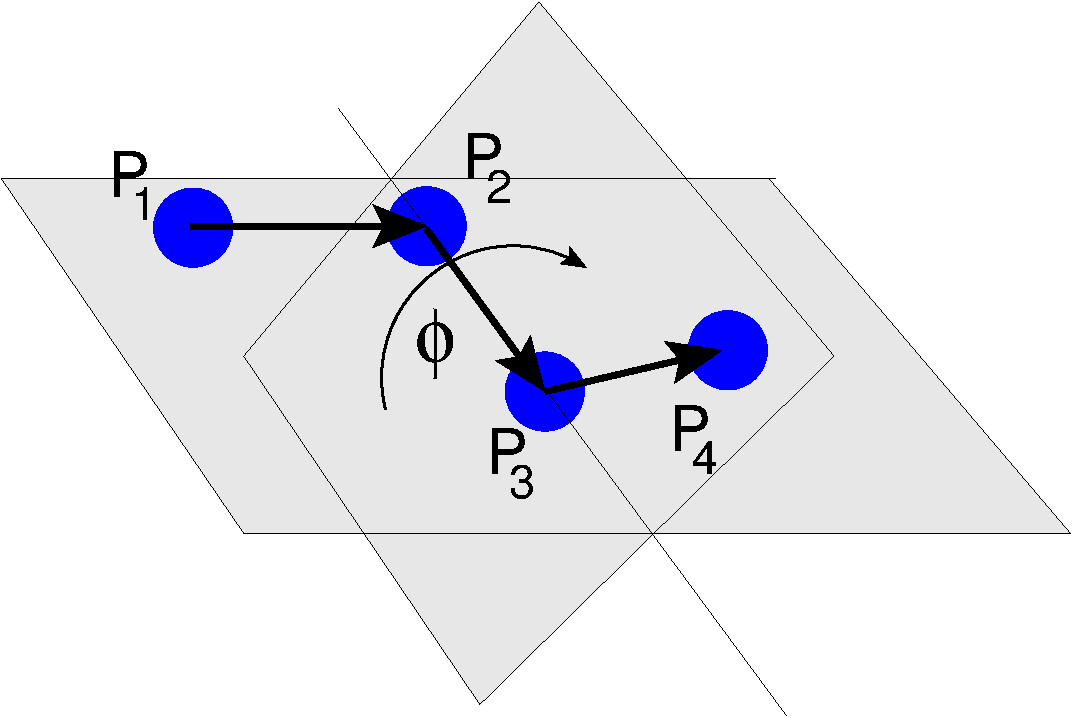
\includegraphics[height=8em]{figures/dihedral-angle.pdf}
\end{center}
Together with appropriate Lennard-Jones interactions, this potential can mimic a
large number of atomic torsion potentials.

\subsection{Tabulated bond interactions}
\index{tabulated bond interactions|mainindex}
\index{interactions!tabulated bond|mainindex}

\begin{essyntax}
    \variant{1} inter \var{bond_type_number}
    tabulated bond \var{filename}
    \variant{2} inter \var{bond_type_number}
    tabulated angle \var{filename}
    \variant{3} inter \var{bond_type_number}
    tabulated dihedral \var{filename}
\end{essyntax}

This creates a bond type with identificator \var{bond_type_number} with a
two-body bond length (\variant{1}), three-body angle (\variant{2}) or four-body
dihedral (\variant{3}) tabulated potential. The tabulated forces and energies
have to be provided in a file \var{filename}, which is formatted identically as
the files for non-bonded tabulated potentials (see
section\ref{sec:tabnonbonded}).

The potential is calculated as follows:
\begin{itemize}
\item Variant~\variant{1} is a two body interaction depending on the distance of
  two particles. The force acts in the direction of the connecting vector
  between the particles. The bond breaks above the tabulated range, but for
  distances smaller than the tabulated range, a linear extrapolation based on
  the first two tabulated force values is used.
\item Variant~\variant{2} is a three-body angle interaction similar to the
  \texttt{angle} potential (see section~\ref{sec:angle}).  It is assumed that
  the potential is tabulated for all angles between 0 and $ \pi $, where 0
  corresponds to a stretched polymer, and just as for the tabulated pair
  potential, the forces are scaled with the inverse length of the connecting
  vectors. The force on particles $p_1$ and $p_3$ (in the notation of
  section~\ref{sec:angle}) acts perpendicular to the connecting vector between
  the particle and the center particle $p_2$ in the plane defined by the three
  particles. The force on the center particle $p_2$ balances the other two
  forces.
\item Variant~\variant{3} tabulates a torsional dihedral angle potential (see
  section~\ref{sec:dihedral}). It is assumed that the potential is tabulated for
  all angles between 0 and $2\pi$. \em{This potential is not tested yet! Use on
    own risk, and please report your findings and eventually necessary fixes.}
\end{itemize}

\subsection{Virtual bonds}

\begin{essyntax}
  inter \var{bond_type_number} virtual_bond
\end{essyntax}

This creates a virtual bond type with identificator \var{bond_type_number}, \ie
a pair bond without associated potential or force. It can used to specify
topologies and for some analysis that rely on bonds, or \eg for bonds that
should be displayed in VMD.

\section{Coulomb interaction}
\label{sec:inter-electrostatics}
\index{Coulomb interactions|mainindex}
\index{interactions!Coulomb|mainindex}

Electrostatic interactions are very computation time-intensive. \es{} features
some state-of-the-art algorithms to deal with these interactions as efficiently
as possible, but almost all of them require some knowledge to use them properly.
Uneducated use can result in completely unphysical simulations.

\begin{essyntax}
  \variant{1} inter coulomb 0.0
  \variant{2} inter coulomb \opt{\var{$l_B$} \var{method}} \opt{\var{parameters}}
\end{essyntax}

This command defines how \es{} deals with electrostatic interactions. Variant
\variant{1} completely disables Coulomb interactions hence deactivating the
electrostatic subsystem, while variant \variant{2} sets up one of the methods
described below to treat electrostatic interactions. \var{$l_B$} denotes the
Bjerrum length, which measures the strength of the electrostatic interaction.
For a pair of particles at distance $r$ with charge $q$ each, the interaction is given by
\begin{equation}
  U^C(r)=l_B k_B T\frac{q^2}{r}.
\end{equation}
Using the electrostatic interaction also requires to assign charges to the
particles. This is done using the \texttt{part} command to set the charge
\texttt{q}, \eg

\begin{tclcode}
  inter coulomb 1.0 p3m tune accuracy 1e-4
  part 0 q 1.0; part 1 q -1.0
\end{tclcode}

When not given a method or \texttt{0.0}, \texttt{inter coulomb} returns the
current parameters of the coulomb interaction as a tcl-list using the same
syntax as used to setup the method, \eg

\begin{tclcode}
  {coulomb 1.0 p3m 7.75 8 5 0.1138 0.0}
  {coulomb epsilon 0.1 n_interpol 32768 mesh_off 0.5 0.5 0.5}
\end{tclcode}

\subsection{P3M}
\index{P3M method|mainindex}
\index{interactions!P3M|mainindex}

\begin{essyntax}
  inter coulomb p3m \var{r_cut} \var{mesh} \var{cao} \var{alpha}
\end{essyntax}

Activates the P3M method to handle the Coulomb
interaction
\begin{equation}
  U^{C-P3M} = \ell_B k_B T \frac{q_1 q_2}{r}
\end{equation}

Here $\ell_B = e_o^2 / (4 \pi \epsilon k_B T)$ is the Bjerrum length.
Make sure that you know the relevance of the P3M parameters before
using P3M! If you are not sure, read the following references \cite{ewald21,hockney88,kolafa92,deserno98,deserno98a,deserno00,deserno00a}.

\subsubsection{Tuning P3M}
\begin{essyntax}
  inter coulomb p3m \alt{tune \asep tunev2}
  accuracy \var{accuracy}\\
  \opt{r_cut \var{r_cut}}
  \opt{mesh \var{mesh}}
  \opt{cao \var{cao}}
  \opt{alpha \var{alpha}}
\end{essyntax}

\todo{Insert docs from \texttt{p3m.h}}

Make sure you know how to tune p3m parameters before using the
automatic tuning feature. Details are described in the documentation
of P3M_tune_parameters rsp P3M_adaptive_tune_parameters in source file p3m.h.

The function utilizes the analytic expression of the error estimate for the P3M method in the book of Hockney and Eastwood (\cite{hockney88} Eqn. 8.23) in order to obtain the rms error in the force for a system of N randomly distributed particles in a cubic box. For the real space error the estimate of Kolafa and Perram\cite{kolafa92} is used.

The two tuning methods follow different methods for determining the
optimal parameter. While the \keyword{tune} version simply tests
different values on a grid in the parameter space, the
\keyword{tunev2} version uses a bisection to determine the optimal
parameters. In general, for small systems the \keyword{tune} version
is faster, while for large systems \keyword{tunev2} is faster. The
results of \keyword{tunev2} are always at least as good as the
parameters achievable from the \keyword{tune} version, and normally
the obtained accuracy is much closer to the desired value.

During execution the tuning routines report the parameter sets tested, the corresponding k-space and real-space errors and timings needed for force calculations (the setmd variable \var{timings} controls the number of test force calculations). Since the error depends on \var{r_cut}/\var{box_l} and \var{alpha}\var{box_l} the output is given in these units, called \var{r_cut_iL} and \var{alpha_L}.

Note that any previous settings of \var{r_cut}, \var{cao} and
\var{mesh} will be remembered. So if you want to retune your
electrostatics, \eg after a major system change, you should use
\begin{code}
inter coulomb \var{bjerrum} p3m tune accuracy \var{acc} r_cut 0 mesh 0 cao 0
\end{code}

Some additional p3m parameters have preset value
\begin{tclcode}
 epsilon = metallic
\end{tclcode}
The dielectric constant of the surrounding medium, metallic
(i.e.infinity) or some finite positive number.
\begin{tclcode}
 n_interpol = 32768
\end{tclcode}
Number of interpolation points for the charge assignment function.
When this is set to 0, interpolation is turned off.
\begin{tclcode}
 mesh_off = 0.5 0.5 0.5
\end{tclcode}
Offset of the first mesh point from the lower left corner of the
simulation box in units of the mesh constant. As soon as p3m is turned
on the additional parameters can be changed with:
\begin{code}
inter coulomb \var{parameter_name} \var{value}+
\end{code}


\subsection{Debye-H\"uckel potential}
\index{Debye-H\"uckel potential|mainindex}
\index{interactions!Debye-H\"uckel|mainindex}

\begin{essyntax}
  inter coulomb dh \var{kappa} \var{r_cut}
\end{essyntax}
\[ U^{C-DH} = \ell_B k_B T \frac{q_1 q_2 exp(-\kappa r)}{r} \]

For

\[ \kappa = 0 \]

this corresponds to the plain coulomb potential.

\subsection{MMM2D}
\index{MMM2D method|mainindex}
\index{interactions!MMM2D|mainindex}

\begin{essyntax}
 inter coulomb mmm2d \var{maximal_pairwise_error} \opt{\var{fixed_far_cutoff}}
\end{essyntax}
MMM2D coulomb method for systems with periodicity 1 1 0. Needs the
layered cell system. The performance of the method depends on the
number of slices of the cell system, which has to be tuned manually.
It is automatically ensured that the maximal pairwise error is smaller
than the given bound. The far cutoff setting should only be used for
testing reasons, otherwise you are more safe with the automatical
tuning. If you even don't know what it is, do not even think of
touching the far cutoff. For details on the MMM family of algorithms,
refer to appendix \vref{chap:mmm}.

\subsection{MMM1D}
\index{MMM1D method|mainindex}
\index{interactions!MMM1D|mainindex}

\begin{essyntax}
  \variant{1}
  inter coulomb mmm1d \var{switch_radius}
  \opt{\var{bessel_cutoff}} \var{maximal_pairwise_error}

  \variant{2}
  inter coulomb mmm1d tune \var{maximal_pairwise_error}
\end{essyntax}
MMM1D coulomb method for systems with periodicity 0 0 1. Needs the
nsquared cell system (see section \vref{sec:cell-systems}). The first
form sets parameters manually. The switch radius determines at which
xy-distance the force calculation switches from the near to the far
formula. If the Bessel cutoff is not explicitly given, it is
determined from the maximal pairwise error, otherwise this error only
counts for the near formula. The second, tuning form just takes the
maximal pairwise error and tries out a lot of switching radii to find
out the fastest one. If this takes too long, you can change the value
of the setmd variable "timings" which controls the number of test
force calculations. For details on the MMM family of algorithms,
refer to appendix \vref{chap:mmm}.

\subsection{Maggs' method}
\index{Maggs' method|mainindex}
\index{interactions!Maggs' method|mainindex}

\begin{essyntax}
  inter coulomb
  maggs \var{f_mass} \var{mesh} \var{field_friction}
  \opt{yukawa \var{kappa} \var{r_cut}}
\end{essyntax}

This is an implementation of the instantaneous 1/r Coulomb interaction

\[ U = \ell_B k_B T \frac{q_1 q_2}{r} \]

as the potential of mean force between charges which are dynamically
coupled to a local electromagnetic field.

\var{f_mass} is the mass of the field degree of freedom and equals to
the square root of the inverted speed of light.

\var{mesh} is the number of mesh points for the interpolation of the
electromagnetic field

\var{field_friction} value of the friction coefficient for the
transversal field degrees of freedom (reserved for future
developments)

Unphysical self--energies that arise as a result of the lattice
interpolation of charges, are corrected by a subtraction scheme based
either on the exact lattice Green's function or the combination of the
direct subtraction scheme plus the Yukawa subtraction scheme (second
method).

For the case of Yukawa screened simulation (second method) one has to
enter screening parameter \var{kappa} and the cut-off of the Yukawa
potential \var{r_cut}.

\subsection{ELC}
\index{ELC method|mainindex}
\index{interactions!ELC method|mainindex}

\begin{essyntax}
  inter coulomb elc \var{maximal_pairwise_error} \var{gap_size}
  \opt{\var{far_cutoff}}
\end{essyntax}
This is a special procedure that converts a 3d method, \ie P3M at the
moment, to a 2d method, in computational order N. This is definitely
faster than MMM2D for larger numbers of particles (>400 at reasonable
accuracy requirements). The maximal pairwise error is the LUB error of
the force between any two charges without prefactors (see the papers).
The gap size gives the height of the empty region between the system
box and the neighboring artificial images (again, see the paper).
\es{} does not make sure that the gap is actually empty, this is the
users responsibility. The method will compute fine of the condition is
not fulfilled, however, the error bound will not be reached. Therefore
you should really make sure that the gap region is empty (e. g. by
constraints). The far cutoff finally is only intended for testing and
allows to directly set the cutoff. In this case, the maximal pairwise
error is ignored. The periodicity has to be set to 1 1 1 still, and
the 3d method has to be set to epsilon metallic, i.e.  metallic
boundary conditions. For details, see appendix \vref{chap:mmm}.

Make sure that you read the papers on ELC before using it !!!
\todo{references}

\section{Other interaction types}
\label{sec:inter-other}

\subsection{Fixing the center of mass}
\begin{essyntax}
  inter \var{particle_type_number1} \var{particle_type_number1}
  comfixed \var{comfixed_flag}
\end{essyntax}
This interaction type applies a constraint on particles of type
\var{particle_type_number1} such that during the integration the
center of mass of these particles is fixed. This is accomplished as
follows: The sum of all the forces acting on particles of type
\var{particle_type_number1} are calculated. These include all the
forces due to other interaction types and also the thermostat. Next a
force equal in magnitude, but in the oppositte direction is applied on
the particles. This force is divided equally on all the particles of
type \var{particle_type_number1}, since currently there is no mass
concept in \es. Note that the syntax of the declaration of comfixed
interaction requires the same particle type to be input twice. If
different particle types are given in the input, the program exits
with an error message. The \var{comfixed_flag} can be set to 1 (which
turns on the interaction) or 0 (to turn off the interaction).

\subsection{Pulling particles apart}
\begin{essyntax}
  inter \var{particle_type_number1} \var{particle_type_number2}\\
  comforce \var{comforce_flag} \var{comforce_dir} \var{comforce_force}
  \var{comforce_fratio}
\end{essyntax}
The comforce interaction type enables one to pull away particle groups
of two different types. It is mainly designed for pulling experiments
on bundles. Within a bundle of molecules of type number 1 (t1) lets
mark one molecule as of type 2 (t2). Using comforce one can apply a
force such that t2 can be pulled away from the bundle. The
\var{comforce_flag} is set to 1 to turn on the interaction, and to 0
otherwise. The pulling can be done in two different directions. Either
parallel to the major axis of the bundle ( \var{comforce_dir} = 0) or
perpendicular to the major axis of the bundle (\var{comforce_dir} =
1). \var{comforce_force} is used to set the magnitude of the force.
\var{comforce_fratio} is used to set the ratio of the force applied on
particles of t1 vs t2. This is useful if one has to keep the total
applied force on the bundle and on the target molecule the same. A
force of magnitude \var{comforce_force} is applied on t2 particles,
and a force of magnitude (\var{comforce_force} *
\var{comforce_fratio}) is applied on t1 particles.

%%% Local Variables:
%%% mode: latex
%%% TeX-master: "ug"
%%% End:
